\documentclass[conference]{IEEEtran}

\usepackage{cite}
\usepackage{amsmath,amssymb,amsfonts}
\usepackage{graphicx}
\usepackage{booktabs}
\usepackage{url}
\usepackage{hyperref}
\usepackage{float}
\usepackage{adjustbox}

\title{An Explainable Multi-Mode Board Game Recommendation System Using Content Similarity, Sentiment Analysis, and Popularity Signals}

\author{
\IEEEauthorblockN{Maximilliano Felix Gunawan}
\IEEEauthorblockA{
Department of Computer Science and Information Engineering\\
Asia University, Taiwan\\
Email: maxfelix05@gmail.com
}
}


\begin{document}


\maketitle

\begin{abstract}
    
    Board games have experienced significant growth in popularity, resulting in increasingly large and complex game catalogs that make game discovery difficult for players. Traditional recommendation approaches often rely heavily on collaborative filtering, which suffers from sparsity and cold-start limitations when user interaction data is limited. To address these challenges, this study proposes an explainable hybrid board game recommendation system that combines content similarity, sentiment analysis, and popularity signals to support multiple recommendation modes.
    
    The proposed system integrates textual game descriptions, gameplay traits, user review sentiment, and popularity-based information to generate recommendations through title-based, trait-based, and combined recommendation modes. Content representations were generated using TF-IDF and sentence-transformer embeddings, while sentiment scores were derived from transformer-based review analysis. The system was evaluated using a filtered subset of the BoardGameGeek dataset containing over 21,000 board games and millions of user ratings and reviews.
    
    Experimental evaluation was conducted using Recall@K and NDCG@K metrics under a holdout-based recommendation setting. Results show that the title-based recommendation mode achieved the strongest quantitative performance, particularly in Recall@10 and NDCG@10, while the combined mode provided more flexible discovery capabilities by incorporating both seed-game similarity and user-selected gameplay traits. In contrast, the trait-based mode demonstrated substantially weaker retrieval effectiveness, highlighting the limitations of sparse trait-only recommendation strategies.
    
    The findings suggest that explainable content-oriented recommendation systems can provide practical and effective support for board game discovery without relying exclusively on collaborative filtering. The proposed framework offers a lightweight and interpretable alternative for hobby-domain recommendation systems while also identifying important limitations and opportunities for future improvement.
    
\end{abstract}

\begin{IEEEkeywords}
Recommender Systems, Board Game Recommendation, Explainable Recommendation, Content-Based Filtering, Sentiment Analysis, Hybrid Recommendation, BoardGameGeek
\end{IEEEkeywords}
\section{Introduction}

Board games have experienced significant growth in popularity over the past decade, resulting in increasingly large and complex game catalogs on online platforms such as BoardGameGeek (BGG). As the number of available games continues to expand, users often face difficulties in discovering games that match their preferences, gameplay styles, and thematic interests. This creates a recommendation challenge in which systems must balance personalization, relevance, diversity, and explainability.

Traditional recommendation systems commonly rely on collaborative filtering techniques, which generate recommendations based on user interaction patterns and rating similarities. Although collaborative filtering has shown strong performance in many domains, it suffers from several important limitations. One major issue is the cold-start problem, where newly added games or users with limited interaction history cannot be effectively recommended. In addition, sparse rating distributions may reduce recommendation quality and system reliability.

Content-based recommendation approaches attempt to address some of these limitations by utilizing item attributes such as descriptions, mechanics, categories, and themes. However, content-only systems often fail to capture qualitative user opinions and emotional responses toward games. Meanwhile, popularity-based approaches may over-recommend highly popular games while ignoring niche preferences and personalized interests.

To address these challenges, this paper proposes an explainable hybrid board game recommendation system that combines multiple recommendation signals into a unified framework. The proposed system integrates content similarity, sentiment analysis derived from user reviews, and popularity information to generate more relevant and interpretable recommendations. Furthermore, the system supports multiple recommendation modes, including title-based recommendations, trait-based recommendations, and combined hybrid recommendations.

The primary contributions of this paper are as follows:

\begin{itemize}
    \item Development of a hybrid recommendation framework combining content similarity, sentiment signals, and popularity metrics.
    
    \item Implementation of explainable recommendation outputs that provide interpretable recommendation reasoning.
    
    \item Support for multiple recommendation modes, including title-based, trait-based, and combined recommendations.
    
    \item Evaluation of recommendation performance using Recall@K and NDCG@K metrics under different recommendation scenarios.
\end{itemize}

The remainder of this paper is organized as follows. Section II reviews related work in recommendation systems and sentiment-aware recommendation approaches. Section III describes the proposed methodology and recommendation architecture. Section IV presents the experimental evaluation and performance analysis. Section V discusses the findings, limitations, and implications of the proposed system. Finally, Section VI concludes the paper and suggests directions for future work.

\section{Related Work}

Recommendation systems have been widely studied as a solution for helping users discover relevant items in large information spaces. Collaborative filtering is one of the most established recommendation approaches and relies on user-item interaction patterns to identify similarities between users or items. Su and Khoshgoftaar \cite{su2009survey} provide a broad survey of collaborative filtering techniques, highlighting their effectiveness as well as their limitations, including rating sparsity and cold-start problems. Herlocker et al. \cite{herlocker2004evaluating} further emphasize the importance of proper evaluation methods when assessing collaborative filtering systems.

Content-based recommendation systems address some of these limitations by recommending items based on item attributes rather than user interaction histories. Pazzani and Billsus \cite{pazzani2007content} describe how content-based systems use textual and metadata features to model item similarity. In the context of board games, this approach is especially relevant because games often contain rich descriptive information, including descriptions, mechanics, categories, themes, and complexity indicators. However, content-based systems may be limited when item metadata does not fully capture user experience or subjective preference.

Hybrid recommendation systems combine multiple recommendation strategies to improve robustness and recommendation quality. Burke \cite{burke2002hybrid} presents hybrid recommender systems as a way to reduce the weaknesses of individual recommendation approaches by combining different sources of evidence. More recent surveys also show that hybrid approaches remain important across different application domains because they can integrate collaborative, content-based, and contextual signals \cite{ko2022survey}. This motivates the design of the proposed system, which combines content similarity, sentiment information, and popularity signals.

Sentiment-aware recommendation systems incorporate user opinions from reviews to improve recommendation relevance. Wang et al. \cite{wang2017location} demonstrate the usefulness of sentiment information in recommender systems by integrating sentiment with contextual recommendation signals. Da'u and Salim \cite{da2019sentiment} also show that sentiment-aware models can enhance recommendation performance by capturing opinion-oriented information from review text. For board game recommendations, sentiment is valuable because user reviews often describe enjoyment, difficulty, replayability, and perceived game quality beyond numerical ratings.

Explainability has also become an important direction in recommender system research. Zhang and Chen \cite{zhang2020explainable} argue that explainable recommendation systems can improve user trust, transparency, and decision support. Chatti et al. \cite{chatti2024visualization} further discuss the role of visualization in recommendation explainability. This is important for board game discovery because users may want to understand why a specific game is recommended, such as shared mechanics, similar themes, positive sentiment, or popularity.

Evaluation is another critical aspect of recommender system development. Ranking-based metrics such as Recall@K and NDCG@K are commonly used to assess whether relevant items appear near the top of a recommendation list. Radlinski and Craswell \cite{radlinski2010comparing} compare the sensitivity of information retrieval metrics, while Sakai and Kando \cite{sakai2008information} discuss evaluation metrics under incomplete relevance assessments. These studies support the use of ranking-oriented evaluation for recommendation tasks where the order of suggested items is important.

Based on the reviewed literature, several gaps remain relevant to board game recommendation. Collaborative filtering methods may struggle under sparse user interaction data, while pure content-based systems may ignore subjective user sentiment. Popularity-based recommendations are simple and robust but may overemphasize mainstream games. Existing studies also often focus on algorithmic accuracy without providing flexible query modes and interpretable explanations for end users. Therefore, this paper proposes an explainable hybrid board game recommendation system that integrates content similarity, sentiment signals, and popularity information while supporting title-based, trait-based, and combined recommendation modes.

\section{Methodology}

This section describes the dataset, feature engineering process, recommendation architecture, and evaluation pipeline used in the proposed hybrid board game recommendation system.

\begin{figure}[H]
\centering
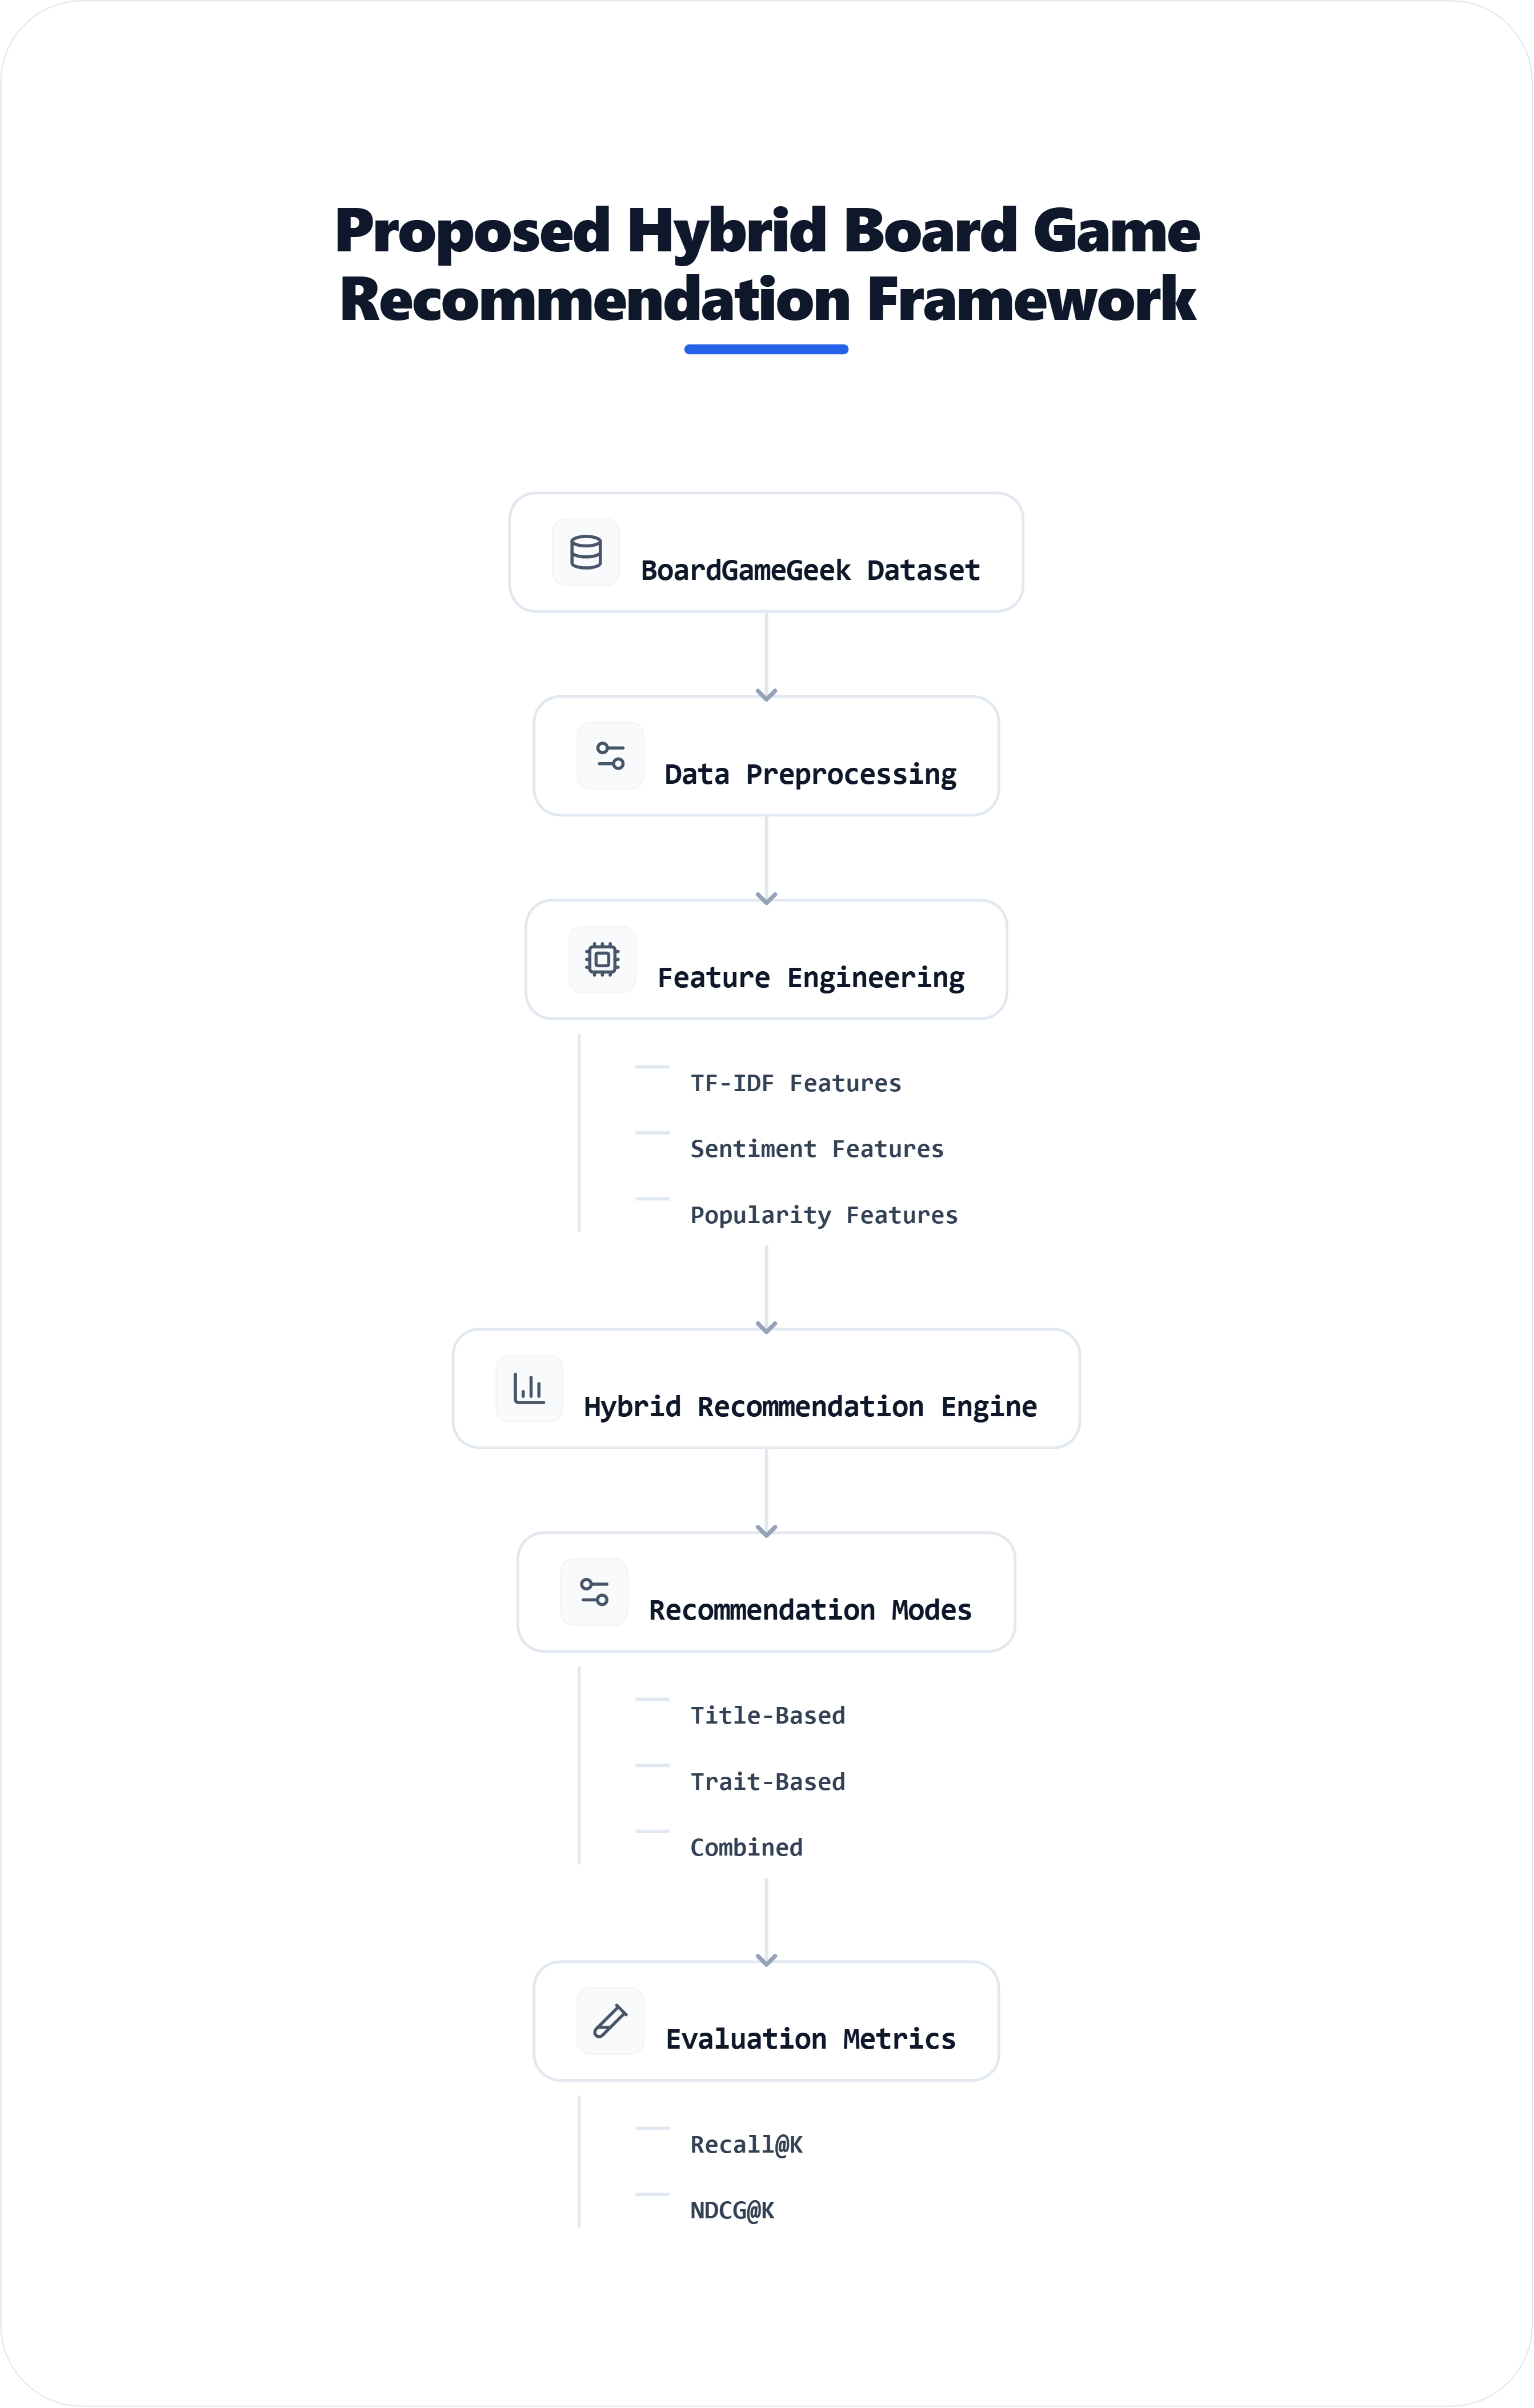
\includegraphics[width=0.50\textwidth]{images/architecture.png}
\caption{Proposed Hybrid Board Game Recommendation Framework}
\label{fig:architecture}
\end{figure}

\subsection{Dataset Description}

This study utilized publicly available board game data collected from the BoardGameGeek (BGG) platform. The dataset contains board game metadata, user ratings, and textual user reviews. After preprocessing and filtering, the final dataset included over 21,000 board games and millions of user rating interactions.

The dataset preprocessing stage involved removing incomplete records, filtering games with insufficient metadata, and cleaning textual review content. Board game attributes such as categories, mechanics, themes, descriptions, complexity ratings, and user rating statistics were retained for recommendation modeling.

User rating data was additionally filtered to reduce sparsity and improve evaluation consistency. The final processed interaction dataset contained approximately 18.7 million valid user ratings after preprocessing.

The evaluation subset was constructed using a random holdout strategy applied to filtered user interaction data. Users with insufficient rating activity were excluded to improve evaluation consistency. For each sampled user, positively rated games were randomly divided into seed-game inputs and held-out relevance targets used during evaluation.

Textual review data was used for sentiment analysis, while game descriptions, categories, and mechanics were used for content-based similarity modeling. The processed dataset was then used to support title-based, trait-based, and combined recommendation experiments.

\subsection{Feature Engineering}

Feature engineering was performed to extract meaningful recommendation signals from board game metadata and review information. The proposed system combines content similarity features, sentiment features, and popularity indicators.

\subsubsection{Content Representation}

Content-based similarity was computed using both TF-IDF vectorization and sentence-transformer embeddings derived from board game descriptions and metadata. Textual attributes including game descriptions, mechanics, and categories were combined into a unified textual representation for each game.

TF-IDF vectorization was used to capture keyword-level similarity, while semantic embeddings generated using the \texttt{all-MiniLM-L6-v2} sentence-transformer model were used to capture higher-level semantic relationships between games. Cosine similarity was then applied to compute pairwise similarity scores between board games.

\subsubsection{Trait Extraction}

Trait-based recommendation utilized structured board game attributes such as mechanics, categories, player count, complexity level, and thematic tags. Trait overlap between games was computed using shared attribute matching, allowing the system to support exploratory recommendation scenarios based on user-selected gameplay preferences.

Trait matching was implemented as a soft overlap mechanism rather than a strict binary filter. Games sharing a larger proportion of relevant gameplay traits received higher trait similarity scores.

\subsubsection{Sentiment Analysis}

User review sentiment was incorporated as an additional recommendation signal. Sentiment scores were generated using the HuggingFace transformer pipeline with the DistilBERT SST-2 sentiment classification model (\texttt{distilbert-base-uncased-finetuned-sst-2-english}) applied to textual user reviews collected from BoardGameGeek.

Individual review sentiment predictions were aggregated at the game level by averaging review sentiment scores associated with each board game. The resulting sentiment values were normalized before integration into the hybrid recommendation framework.

\subsubsection{Popularity Signal}

Popularity-based information was incorporated using aggregate user rating statistics. Popularity scores were derived from a combination of average user rating and rating count, allowing highly rated and widely played games to receive stronger popularity signals.

To prevent popularity values from dominating the hybrid recommendation score, popularity features were normalized prior to score combination.

\subsection{Score Normalization}

The recommendation framework combines multiple heterogeneous signals, including content similarity, trait overlap, sentiment scores, and popularity statistics. Because these components operate on different numerical scales, normalization was applied before score aggregation to ensure balanced contribution within the hybrid recommendation framework.

Content similarity scores computed using cosine similarity naturally fall within the range of [0,1] and therefore required no additional normalization. Trait overlap scores were similarly scaled to the [0,1] range based on proportional shared attribute matching.

Popularity scores derived from rating counts and average ratings were normalized using min-max normalization to prevent highly popular games from dominating the recommendation score. Aggregated sentiment scores were also normalized prior to integration into the final recommendation formula.

\subsection{Hybrid Recommendation Formula}

The final recommendation score was computed using a weighted combination of content similarity, trait similarity, sentiment score, and popularity score:

\begin{equation}
Score = w_1 C + w_2 T + w_3 S + w_4 P
\end{equation}

where:

\begin{itemize}
    \item $C$ represents content similarity,
    \item $T$ represents trait overlap similarity,
    \item $S$ represents normalized sentiment score,
    \item $P$ represents normalized popularity score.
\end{itemize}

The weighting configuration used in this study was manually tuned to prioritize semantic similarity while still incorporating supporting sentiment and popularity signals. The weights used throughout the experiments were:

\begin{itemize}
    \item $w_1 = 0.50$ (Content Similarity)
    \item $w_2 = 0.20$ (Trait Similarity)
    \item $w_3 = 0.15$ (Sentiment Score)
    \item $w_4 = 0.15$ (Popularity Score)
\end{itemize}

Content similarity received the highest weight because semantic similarity between games was considered the primary recommendation objective within the proposed discovery-oriented recommendation framework.

\subsection{Recommendation Modes}

The proposed framework supports three recommendation modes designed for different board game discovery scenarios.

\subsubsection{Title-Based Recommendation}

The title-based mode generates recommendations using similarity relationships derived from a selected seed board game. This mode primarily emphasizes semantic content similarity and achieved the strongest quantitative performance during evaluation.

\subsubsection{Trait-Based Recommendation}

The trait-based mode allows users to explore games using gameplay-related characteristics such as mechanics, themes, complexity level, and player configuration. This mode was designed to support exploratory discovery scenarios where users may not have a specific seed game in mind.

\subsubsection{Combined Recommendation}

The combined recommendation mode integrates both seed-game similarity and trait-based filtering to provide guided discovery recommendations. This mode was intended to balance semantic similarity with user-selected gameplay preferences, enabling more flexible exploration of the board game catalog.

\subsection{Evaluation Strategy}

The recommendation framework was evaluated using a holdout-based recommendation protocol constructed from filtered BoardGameGeek user interaction data.

A subset of 300 users was sampled from the processed rating dataset. For each user, three positively rated board games were selected as seed games, while an additional three positively rated games were withheld as ground-truth relevance targets for evaluation.

Recommendation quality was evaluated using Recall@K and NDCG@K metrics at multiple cutoff levels. A recommendation was considered relevant if a recommended game matched one of the user's held-out positively rated games.

Recall@K was used to measure the proportion of relevant games successfully retrieved within the top-K recommendations, while NDCG@K was used to evaluate ranking quality by assigning higher importance to correctly ranked recommendations appearing earlier in the recommendation list.

\subsection{System Implementation}

The recommendation system was implemented using Python-based data science tools and libraries. Data preprocessing and analysis were performed using Pandas and NumPy, while TF-IDF vectorization and similarity calculations were implemented using Scikit-learn. The user interface prototype was developed using Streamlit to provide interactive recommendation exploration and explainable recommendation outputs.

The system architecture was designed to support modular recommendation experiments and evaluation workflows.

\section{Evaluation}

This section presents the experimental setup, evaluation metrics, baseline methods, and performance analysis used to evaluate the proposed hybrid board game recommendation system.

\subsection{Explainability Example}

To improve recommendation transparency, the proposed system provides lightweight explanation outputs describing why individual board games were recommended. Recommendation explanations are generated using the dominant contributing recommendation signals, including semantic similarity, shared gameplay mechanics, sentiment information, and popularity indicators.

An example recommendation explanation is shown in Table II.

\begin{table}[h]
\centering
\caption{Example Explainable Recommendation Output}
\begin{tabular}{|l|p{5.5cm}|}
\hline
Recommended Game & Explanation \\
\hline
Wingspan & Shared engine-building mechanics, high semantic similarity, and strong positive community sentiment. \\
\hline
Azul & Similar abstract strategy gameplay and comparable player complexity level. \\
\hline
Terraforming Mars & High thematic similarity and strong popularity among strategy game players. \\
\hline
\end{tabular}
\end{table}

\subsection{Evaluation Metrics}

To evaluate recommendation quality, this study utilizes ranking-based evaluation metrics commonly used in recommender systems research, namely Recall@K and Normalized Discounted Cumulative Gain (NDCG@K).

Recall@K measures the proportion of relevant items successfully retrieved within the top-K recommendations. This metric is useful for evaluating whether the recommendation system is capable of retrieving relevant board games for users.

The Recall@K metric is defined as follows:

\begin{equation}
Recall@K =
\frac{\text{Number of Relevant Recommended Items}}
{\text{Total Number of Relevant Items}}
\end{equation}

NDCG@K evaluates ranking quality by assigning higher importance to relevant items appearing near the top of the recommendation list. Unlike Recall@K, NDCG@K considers recommendation ordering and ranking position.

The Discounted Cumulative Gain (DCG) is computed as:

\begin{equation}
DCG@K =
\sum_{i=1}^{K}
\frac{rel_i}{\log_2(i+1)}
\end{equation}

The normalized version is computed as:

\begin{equation}
NDCG@K =
\frac{DCG@K}{IDCG@K}
\end{equation}

where $IDCG@K$ represents the ideal discounted cumulative gain.

These metrics were selected because recommendation ranking quality is important in board game discovery scenarios, where users typically interact with only the top portion of recommendation results.

\subsection{Experimental Setup}

The recommendation experiments were conducted using the processed BoardGameGeek dataset. The dataset was divided into recommendation input data and evaluation targets for ranking analysis.

Several recommendation scenarios were evaluated, including:
\begin{itemize}
    \item Title-based recommendation,
    \item Trait-based recommendation,
    \item Combined hybrid recommendation.
\end{itemize}

The experiments focused primarily on evaluating recommendation ranking quality under sparse user interaction conditions commonly observed in hobby-domain recommendation environments.

Recommendation results were generated using the hybrid scoring framework described in Section III. Different recommendation signals, including content similarity, sentiment information, and popularity indicators, contributed to the final ranking score.

\subsubsection{Popularity-Based Baseline}

The popularity-based baseline recommends games primarily using popularity indicators such as rating count and average rating. This baseline represents a simple recommendation strategy commonly used in many recommendation platforms.

\subsubsection{Content-Based Baseline}

The content-based baseline generates recommendations using textual similarity and metadata similarity without sentiment or popularity integration. This baseline evaluates the contribution of hybrid recommendation components beyond pure content similarity.

\subsection{Experimental Results}

The experimental evaluation focused on comparing the effectiveness of the three proposed recommendation modes under a consistent holdout-based recommendation setting. Recommendation quality was analyzed using Recall@K and NDCG@K metrics across multiple ranking cutoffs.

\begin{figure}[H]
\centering
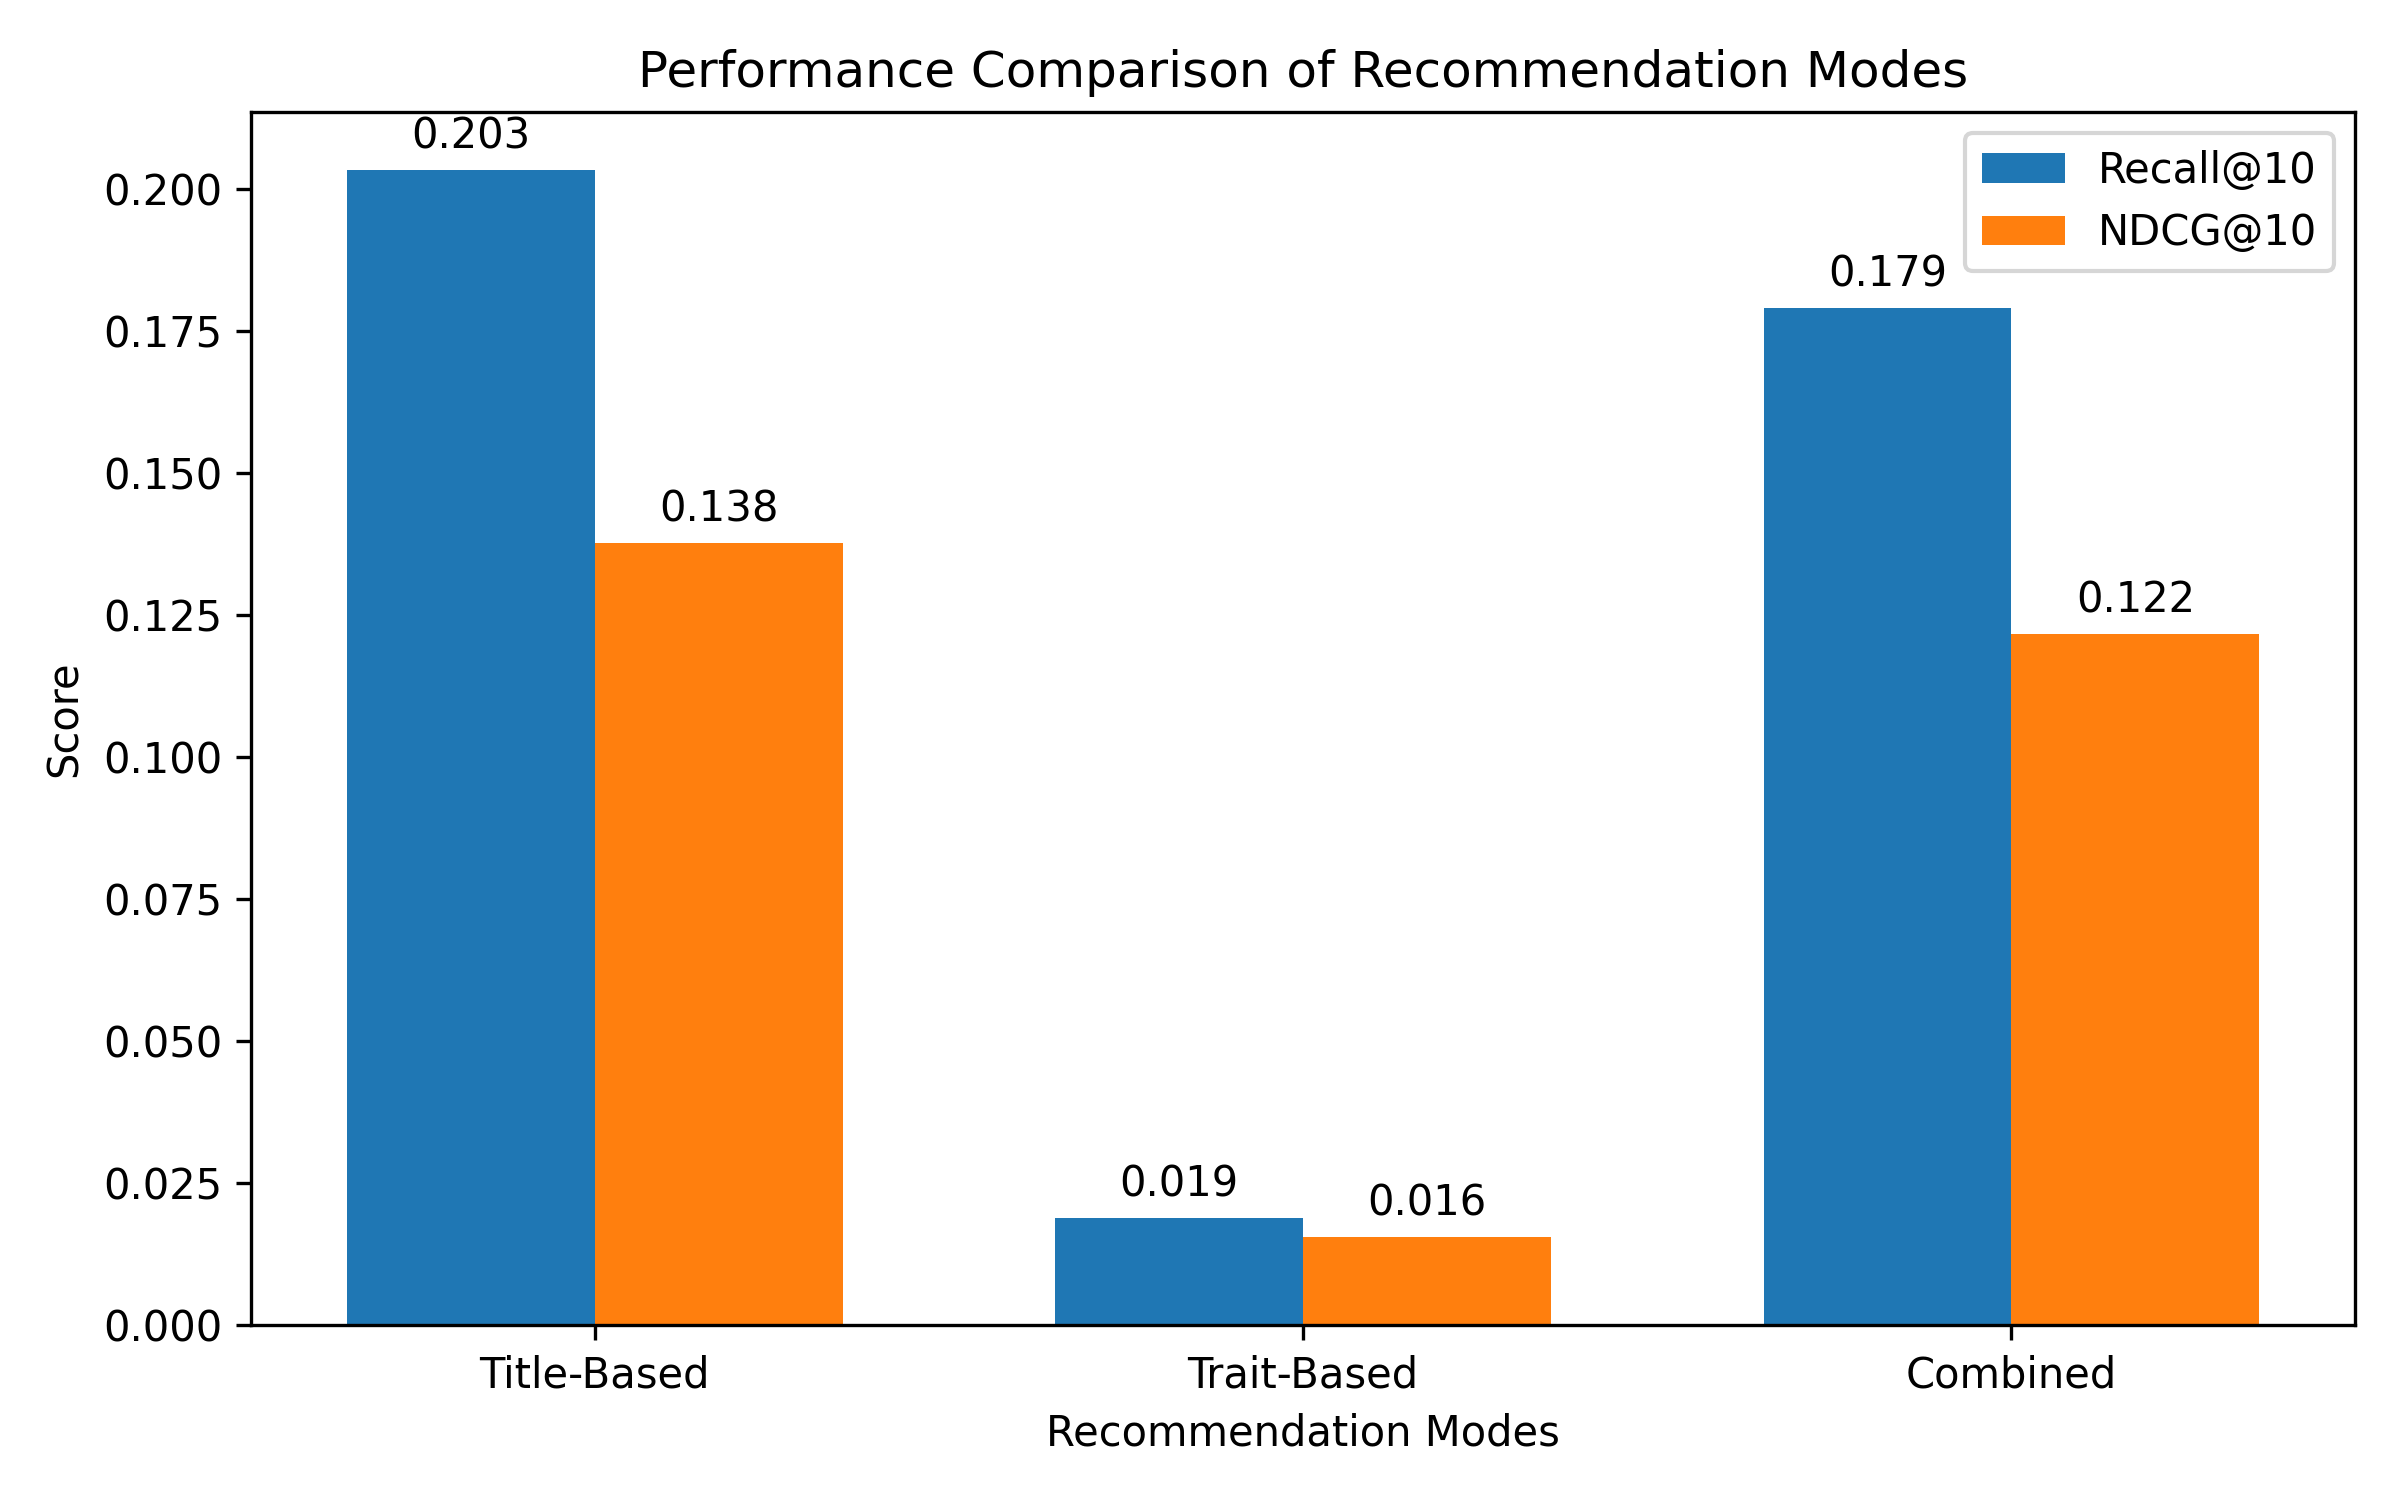
\includegraphics[width=0.55\textwidth]{images/performance_chart.png}
\caption{Performance Comparison of Recommendation Modes}
\label{fig:performance}
\end{figure}

\begin{table}[h]
\centering
\caption{Recommendation Performance Comparison}
\begin{adjustbox}{width=\columnwidth}
\begin{tabular}{lcccccc}
\toprule
Model & Recall@5 & NDCG@5 & Recall@10 & NDCG@10 & Recall@20 & NDCG@20 \\
\midrule
Title-Based & 0.1144 & 0.0977 & 0.2033 & 0.1377 & 0.3011 & 0.1726 \\
Trait-Based & 0.0144 & 0.0137 & 0.0189 & 0.0156 & 0.0367 & 0.0219 \\
Combined & 0.0967 & 0.0846 & 0.1789 & 0.1217 & 0.2822 & 0.1588 \\
\bottomrule
\end{tabular}
\end{adjustbox}
\label{tab:results}
\end{table}

The experimental results demonstrate that the title-based recommendation mode achieved the strongest overall ranking performance across most evaluation metrics. As shown in Table \ref{tab:results}, the title-based approach achieved the highest Recall@10 value of 0.2033 and the highest NDCG@10 value of 0.1377.

The combined recommendation mode also demonstrated strong performance, achieving Recall@10 and NDCG@10 values of 0.1789 and 0.1217 respectively. Although its ranking accuracy was slightly lower than the title-based approach, the combined model provides greater flexibility by integrating both title similarity and gameplay preference constraints.

The trait-based recommendation mode achieved lower ranking performance compared to the other approaches. However, this mode remains useful in situations where users may not know specific board game titles and instead prefer searching through gameplay mechanics, themes, or category preferences.

\subsection{Discussion of Results}

The experimental findings suggest that combining multiple recommendation signals provides advantages over relying on a single recommendation strategy. Content similarity effectively captures gameplay and thematic relationships, while sentiment signals contribute qualitative evaluation information derived from user reviews.

However, several limitations remain. Sparse review information may reduce sentiment reliability for less popular games. In addition, popularity signals may introduce bias toward highly rated mainstream games. Despite these limitations, the proposed hybrid architecture demonstrates improved flexibility, interpretability, and recommendation quality for board game discovery tasks.

\section{Discussion}

The experimental results demonstrate that title-based recommendation achieved the strongest ranking performance among the evaluated recommendation modes. This suggests that providing a specific board game title as a recommendation seed offers strong contextual information for similarity matching. Because board games often contain highly descriptive metadata related to mechanics, themes, complexity, and player interaction, title-based similarity can effectively identify closely related games.

The combined recommendation mode demonstrated moderately strong performance across both Recall@K and NDCG@K metrics while offering greater recommendation flexibility than the purely title-based approach. By integrating seed-game similarity with gameplay preference filtering, the combined framework supports guided discovery scenarios where users may simultaneously consider known favorite games and preferred mechanics, themes, or gameplay styles. Although its quantitative retrieval performance was slightly lower than the title-based mode, the combined approach may provide stronger practical usability for exploratory recommendation tasks.

The trait-based recommendation mode produced substantially lower recommendation performance compared to the other evaluated approaches. One possible explanation is that gameplay traits and category preferences are inherently broader and less semantically specific than title-based similarity representations. As a result, trait-based recommendation generates a larger and more diverse candidate space, increasing ranking difficulty and reducing retrieval precision. Despite these limitations, the trait-based mode remains useful for exploratory recommendation scenarios in which users may not know specific board game titles and instead prefer discovering games through mechanics, themes, complexity levels, or gameplay styles.

The integration of sentiment information contributed additional qualitative recommendation signals derived from user reviews. Unlike pure metadata similarity, sentiment-aware recommendation incorporates subjective user opinions related to enjoyment, replayability, and overall player experience. This improves explainability and allows the recommendation system to incorporate community perception beyond numerical ratings alone.

Despite these strengths, several limitations remain. First, sentiment reliability depends on the availability and quality of user reviews, which may vary significantly across games. Less popular games often contain limited review information, reducing the effectiveness of sentiment-based recommendation signals. Second, popularity features may introduce bias toward highly rated mainstream games while underrepresenting niche or newly released games. Third, the current system does not incorporate collaborative filtering or personalized user interaction modeling, which may further improve recommendation quality in future work.

Future research may explore the integration of collaborative filtering, embedding-based semantic similarity, and large language model (LLM)-based explanation generation. Additional evaluation with real user studies and interactive feedback collection may also improve recommendation personalization and practical deployment readiness.

\section{Conclusion}

This study proposed an explainable hybrid board game recommendation framework that integrates content similarity, gameplay trait matching, sentiment analysis, and popularity-based signals to support multiple recommendation modes for board game discovery. The proposed system was designed as a lightweight and interpretable alternative to recommendation approaches that rely heavily on collaborative filtering and large-scale user interaction history.

Experimental evaluation using Recall@K and NDCG@K demonstrated that the title-based recommendation mode achieved the strongest overall retrieval effectiveness across the evaluated metrics. The combined recommendation mode provided greater flexibility for guided discovery by integrating seed-game similarity with gameplay preference filtering, while the trait-based mode supported exploratory recommendation scenarios despite weaker quantitative performance.

The findings suggest that semantic content similarity remains the most reliable recommendation signal within the proposed framework, while additional signals such as sentiment and gameplay traits contribute useful contextual and explainability-oriented information. The study also highlights the challenges of trait-only recommendation approaches, particularly when semantic contextual information is limited.

Overall, the proposed framework demonstrates that explainable and discovery-oriented recommendation systems can provide practical support for hobby-domain recommendation tasks without requiring fully personalized collaborative filtering architectures. Future work may explore the integration of collaborative filtering, embedding-based semantic retrieval, interactive user feedback, and large language model (LLM)-based explanation generation to further improve recommendation quality and personalization.

\bibliographystyle{IEEEtran}
\bibliography{references}

\end{document}